%%%%%%%%%%%%%%%%%%%%%%%%%%%%%%%%%%%%%%%%%%%%%%%%%%%%%%%%%%%%%%%%%%%%%%%%%%%%%%%
% Chapter 2: Conceptos
%%%%%%%%%%%%%%%%%%%%%%%%%%%%%%%%%%%%%%%%%%%%%%%%%%%%%%%%%%%%%%%%%%%%%%%%%%%%%%%

%++++++++++++++++++++++++++++++++++++++++++++++++++++++++++++++++++++++++++++++
En este capítulo se abordarán todos aquellos conceptos teóricos que han surgido
a lo largo del proyecto y son necesarios para entender correctamente la línea
del trabajo.


%++++++++++++++++++++++++++++++++++++++++++++++++++++++++++++++++++++++++++++++
\section{Visión artificial}
\label{2:sec:1}
%%%%%%%%%%%%%%%%%%%%%%%%%%%%%%%%%%%%%%%%%%%%%%%%%%%%%%%%%%%%%%%%%%%%%%%%%%%%%%%%
% Chapter 2: Conceptos
%%%%%%%%%%%%%%%%%%%%%%%%%%%%%%%%%%%%%%%%%%%%%%%%%%%%%%%%%%%%%%%%%%%%%%%%%%%%%%%%

%++++++++++++++++++++++++++++++++++++++++++++++++++++++++++++++++++++++++++++++
% \section{Visión artificial}
% \label{2:sec:1}
% https://campusvirtual.ull.es/1516/course/view.php?id=202
% https://es.wikipedia.org/wiki/Visi%C3%B3n_artificial
% https://en.wikipedia.org/wiki/Computer_vision
% J. GONZÁLEZ JIMÉNEZ, "Visión Por Computador", Editorial Paraninfo. 2000

La visión artificial por computador, es la disciplina científica que se basa en
la adquisición, procesamiento y análisis de las imágenes que se toman del mundo
real, con el objetivo de obtener información relevante acerca de ellas:
detección de objetos, seguimiento del movimiento, reconocimiento de eventos,
etc. Un ejemplo que podemos ver en nuestro día a día, es la detección de caras
en una escena capturada por una cámara digital o smartphone, mediante el uso de
téncicas de reconocimiento de patrones.

Al igual que sucede en otras áreas de la inteligencia artificial, la visión
artificial tiene como objetivo principal obtener la información explícita y el
significado de la realidad de la misma manera que lo haría un ser biológico.

El avance progresivo del hardware con nuevos procesadores digitales de señales
(DSP) y unidades de procesamiento gráfico (GPU), junto con nuevas tecnologías y
planteamientos de cómputo como la computación paralela, ha permitido que en los
últimos años se haya podido implementar nuevos algortimos más rápidos y
eficientes, necesarios para ser utilizados en ámbitos críticos, como sistemas
en tiempo real.

%+++++++++++++++++++++++++++++++++++++++++++++++++++++++++++++++++++++++++++++++
\subsection{Objetivos}

\textcolor{red}{Lorem ipsum dolor sit amet, consectetur adipisicing elit, sed do
 eiusmod tempor incididunt ut labore et dolore magna aliqua. Ut enim ad minim 
 veniam, quis nostrud exercitation ullamco laboris nisi ut aliquip ex ea commodo 
 consequat. Duis aute irure dolor in reprehenderit in voluptate velit esse cillum
 dolore eu fugiat nulla pariatur. Excepteur sint occaecat cupidatat non proident,
 sunt in culpa qui officia deserunt mollit anim id est laborum.}

\textcolor{red}{Lorem ipsum dolor sit amet, consectetur adipisicing elit, sed do
 eiusmod tempor incididunt ut labore et dolore magna aliqua. Ut enim ad minim 
 veniam, quis nostrud exercitation ullamco laboris nisi ut aliquip ex ea commodo 
 consequat. Duis aute irure dolor in reprehenderit in voluptate velit esse cillum
 dolore eu fugiat nulla pariatur. Excepteur sint occaecat cupidatat non proident,
 sunt in culpa qui officia deserunt mollit anim id est laborum.}

%+++++++++++++++++++++++++++++++++++++++++++++++++++++++++++++++++++++++++++++++
\subsection{Dificultades}
La capacidad visual es uno pilares de la inteligencia humana. Su implementación
en la rotótica supone también un importante avance en la inteligencia
artificial. Sin embargo, mientras que la percepción visual es algo innato y
cotidiano para nosotros, la visión artificial es muy compleja y conlleva muchas
dificultades. Entre las principales dificultades, destacan:

\begin{itemize}
  \item \textbf{Mundo tridimensional:} mientras que las imágenes que se
  obtienen con una cámara son bidimensionales, el mundo que nos rodea no. Es
  necesario realizar las transformaciones correspondientes para obtener valores
  correctos.
  \item \textbf{Zonas de interés:} se necesita extraer elementos de información 
  sutiles en imágenes complejas, por lo que entre tanta información es
  necesario reconocer formas, colores, etc.
  \item \textbf{Carácter dinámico de las escenas:} el mundo está vivo, por lo
  que en las imágenes que se toman muchos elementos están en movimiento. Por 
  otro lado, otros factores como luminosidad, contraste, foco... pueden marcar
  una importante diferencia, y por desgracia, estos factores son variables, no
  se pueden controlar.
\end{itemize}

%+++++++++++++++++++++++++++++++++++++++++++++++++++++++++++++++++++++++++++++++
% \subsection{Reconocimiento}

% Detección de objetos

%+++++++++++++++++++++++++++++++++++++++++++++++++++++++++++++++++++++++++++++++
% \subsection{Motion Analysis}

% Video grabación de imágenes de seguridad

%+++++++++++++++++++++++++++++++++++++++++++++++++++++++++++++++++++++++++++++++
% \subsection{Reconstrucción}

%++++++++++++++++++++++++++++++++++++++++++++++++++++++++++++++++++++++++++++++


%++++++++++++++++++++++++++++++++++++++++++++++++++++++++++++++++++++++++++++++
\section{Visión estéreo}
\label{2:sec:2}
%%%%%%%%%%%%%%%%%%%%%%%%%%%%%%%%%%%%%%%%%%%%%%%%%%%%%%%%%%%%%%%%%%%%%%%%%%%%%%%%
% Chapter 2: Conceptos
%%%%%%%%%%%%%%%%%%%%%%%%%%%%%%%%%%%%%%%%%%%%%%%%%%%%%%%%%%%%%%%%%%%%%%%%%%%%%%%%

%++++++++++++++++++++++++++++++++++++++++++++++++++++++++++++++++++++++++++++++
% \section{Visión estéreo}
% \label{2:sec:2}
% http://vision.deis.unibo.it/~smatt/Seminars/StereoVision.pdf
% http://www.cesfelipesegundo.com/revista/articulos2011/Guerrero,%20J.M.pdf

La visión estereoscópica o visión estéreo, es la técnica capaz de extraer
información tridimensional (profundidad) a partir de la posición relativa de un
objeto en imágenes bidimensionales al ser observado desde distintos ángulo por
dos o más cámaras separadas a una cierta distancia.

%--------------------------------------
\subsection{Calibración}

%--------------------------------------
\subsection{Adquisición}

Usando dos cámaras, el procedimiento a seguir para la adquisición del entorno
es capturar dos imágenes de una misma escena, desde dos cámaras separadas
ligeramente. De esta forma, las imágenes obtenidas, también tendrán un pequeño 
desplazamiento entre sí.

De manera más formal, se obtiene que para cada imagen capturada por las
cámaras, un objeto está en puntos diferentes del plano. Esta triangulazión
entre el punto P y Q y el origen de referencia, provocan una sensación de
profundidad. Mediante el sistema tradicional de una sola cámara, este punto
estaría en las mismas coordenadas.

\begin{figure}[!th]
  \begin{center}
    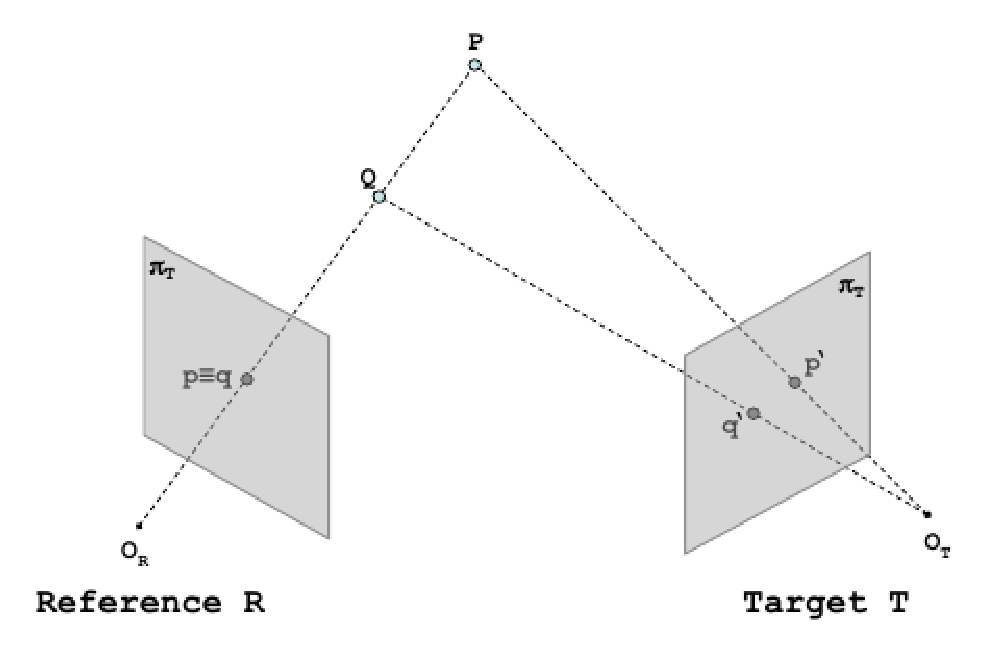
\includegraphics[width=0.7\textwidth]{images/cap2/VisionEstereo.eps}
    \caption{Diferencias entre una y dos cámaras}
    \label{fig:VisionEstereo}
  \end{center}
\end{figure}

Con estos datos, se pueden poner en correspondencia cada punto de ambas
imágenes, para obtener una imagen de disparidad (más información en la sección 
2.2.4).

%--------------------------------------
\subsection{Geometría de las cámaras}
% https://en.wikipedia.org/wiki/Parallax
% http://www.cesfelipesegundo.com/revista/articulos2011/Guerrero,%20J.M.pdf
En función de la posición relativa de las cámaras entre sí, se pueden apreciar
dos métodos principales:

\begin{itemize}
  \item \textbf{Visión paralela:} las cámaras están paralelas entre sí y están
  separadas por una línea horizonal (línea base). El objetivo que visualiza
  cada cámara es perpendicular respecto a la línea base, mientras que las
  líneas de correspondencia que unen los puntos de una imagen respecto a la
  otra son horizontales.

  \begin{minipage}{\linewidth}
      \centering
      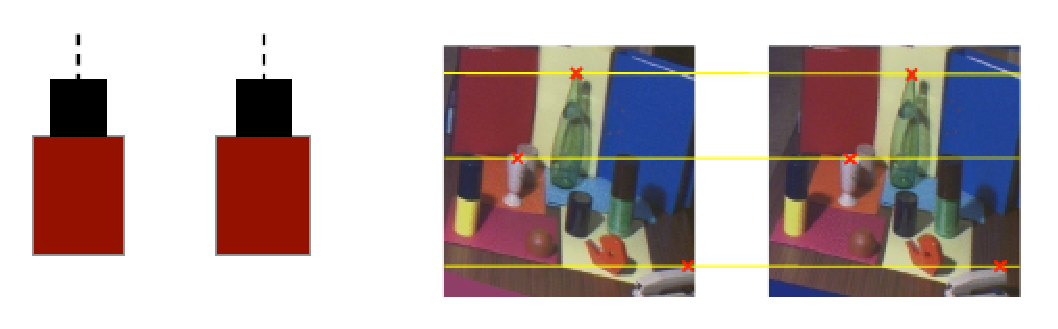
\includegraphics[width=0.7\textwidth]{images/cap2/VisionParalela.eps}
      \captionof{figure}{Visión paralela}
      \label{fig:VisionParalela}
  \end{minipage}

  \item \textbf{Visión cruzada:} las cámaras no están paralelas entre sí,
  tienen una inclinación de tal forma que el objetivo de cada cámara apunta
  hacia el lado contrario de una imagen. Por lo que los ejes ópticos se cruzan
  entre sí. Las líneas de correspondencia, también tienen sufren una
  inclinación.

  \begin{minipage}{\linewidth}
      \centering
      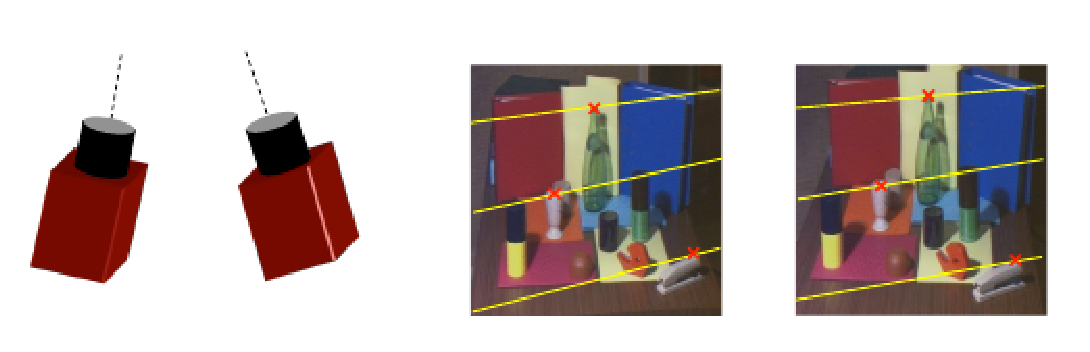
\includegraphics[width=0.7\textwidth]{images/cap2/VisionCruzada.eps}
      \captionof{figure}{Visión cruzada}
      \label{fig:VisionCruzada}
  \end{minipage}
\end{itemize}

% http://vfxio.com/PDFs/Parallel_vs_Converged.pdf
La visión cruzada tiene la desventaja de distorsionar las imágenes capturadas.
En la figura 2.4 se puede observar este efecto al fotografíar un muro de
ladrillos. Sin embargo, dependiendo del tipo de escena que se capture, esta
distorsión puede suponer un problema o no.

\begin{figure}[!th]
  \begin{center}
    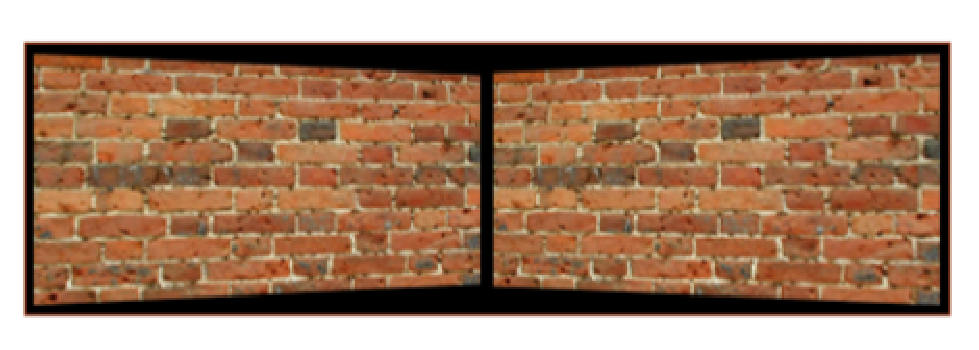
\includegraphics[width=0.5\textwidth]{images/cap2/VisionCruzadaMuro.eps}
    \caption{Muro distorsionado por visión cruzada}
    \label{fig:VisionCruzadaMuro}
  \end{center}
\end{figure}

La visión paralela por su parte, no distorsiona las imágenes capturadas, pero
también cuenta con otra serie de problemas. A pesar de ello, la visión paralela
suele ser la más utilizada para la visión estéreo.

%--------------------------------------
\subsection{Rectificación}
% https://en.wikipedia.org/wiki/Image_rectification

%--------------------------------------
\subsection{Disparidad}
% http://es.slideshare.net/RicardoSnchezCastill/vision-artificial-49264591
% http://stackoverflow.com/questions/17607312/difference-between-disparity-map-and-disparity-image-in-stereo-matching
% http://iie.fing.edu.uy/publicaciones/2005/Lec05a/Lec05a.pdf
La disparidad de dos imágenes establece la correspondencia entre los píxeles o
características que existen entre ambas para obtener la profundidad de la
escena.

El objetivo final es poder construir una \textbf{imagen o mapa de disparidad}.

\begin{figure}[!th]
  \begin{center}
    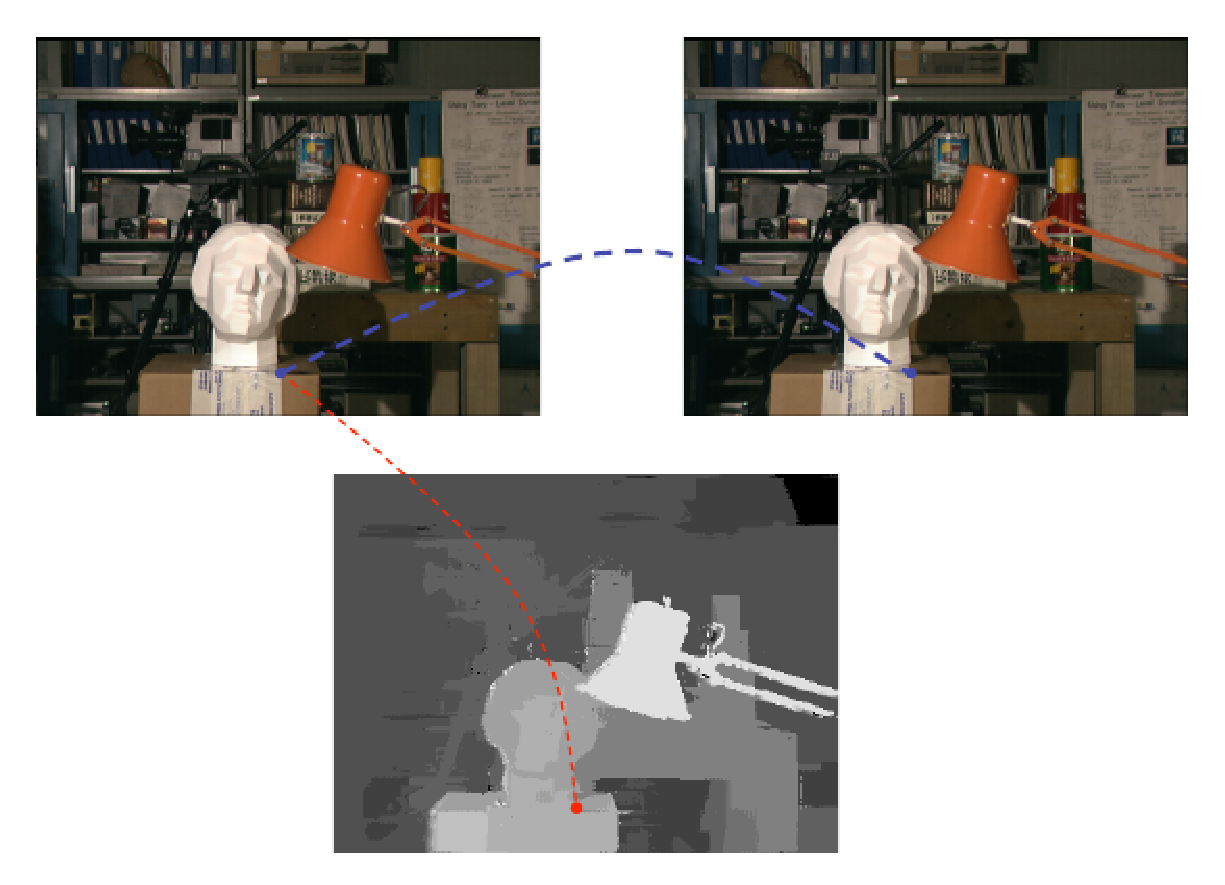
\includegraphics[width=0.7\textwidth]{images/cap2/MapaDisparidad.eps}
    \caption{Mapa de disparidad a partir de imágenes en estéreo}
    \label{fig:MapaDisparidad}
  \end{center}
\end{figure}







% Disparidad....

% http://www.cesfelipesegundo.com/revista/articulos2011/Guerrero,%20J.M.pdf
% http://dmi.uib.es/~abasolo/cursorealidad/paco/Estereoscopia.html


%--------------------------------------
\subsection{Reconstrucción 3D}

%--------------------------------------
\subsection{Aplicaciones}
% https://www.ptgrey.com/tan/10570
La visión artificial resulta de gran utilidad en diferentes áreas de
aplicación, tanto en acciones repetitivas como peligrosas:


\begin{itemize}
  \item \textbf{Inspección y ensamblaje industrial:} el proyecto "Randon Bin
  Picking" (RBP) hace uso de visión estéreo para la búsqueda de piezas entre
  objetos de todo tipo para su rápida recuperación.
  % http://www.worldscientific.com/doi/suppl/10.1142/8766/suppl_file/8766_chap01.pdf
  \item \textbf{Apoyo en el diagnóstico médico:} en las últimas décadas la
  visión artificial se ha hecho un importante en la medicina para detectar,
  analizar y reconstruir la información obtenida.
  % http://www.ri.cmu.edu/pub_files/pub4/matthies_larry_2007_1/matthies_larry_2007_1.pdf
  \item \textbf{Exploración espacial:} en el proyecto de exploración Mars Rover
  (Mars Exploration Rover Mission) tiene como objetivo explorar la superficie
  de Marte en busca de rocas u otros elementos que prueben la existencia de
  agua.
  \item \textbf{Seguimiento (Tracking):} se hace uso en innumerables
  situaciones de carácter estadístico como contar el número o de en áreas de
  vigilancia y seguridad monitorizando trayectorias.
\end{itemize}

%++++++++++++++++++++++++++++++++++++++++++++++++++++++++++++++++++++++++++++++


%++++++++++++++++++++++++++++++++++++++++++++++++++++++++++++++++++++++++++++++
\section{Odometría}
\label{2:sec:3}
%%%%%%%%%%%%%%%%%%%%%%%%%%%%%%%%%%%%%%%%%%%%%%%%%%%%%%%%%%%%%%%%%%%%%%%%%%%%%%%%
% Chapter 2: Conceptos
%%%%%%%%%%%%%%%%%%%%%%%%%%%%%%%%%%%%%%%%%%%%%%%%%%%%%%%%%%%%%%%%%%%%%%%%%%%%%%%%

%++++++++++++++++++++++++++++++++++++++++++++++++++++++++++++++++++++++++++++++
% \section{Odometría}
% \label{2:sec:3}

La odometría es el método que permite estimar la posición de un robot móvil en
el entorno en un momento determinado. 

Cabe recalcar, que la odometría no permite conocer la posición exacta de un
robot, ya que existen muchos factores externos, que provocan errores en la
obtención de los datos de entrada. Estos errores son acumulativos, por lo que
la veracidad de los resultados es inversamente proporcional a la distancia
recorrida de un robot.

A pesar de ello, la odometría ofrece una gran precisión a corto plazo y su
precio de implementación es realmente bajo, por lo que lo convierte en uno de
los pilares básicos para la navegación. 

Dependiendo de la tecnología utilizada para calcular la odometría, se puede 
hablar de diferentes tipos.

%+++++++++++++++++++++++++++++++++++++++++++++++++++++++++++++++++++++++++++++++
\subsection{Odometría mecánica}
La odometría mecánica se base en el estudio del giro de las ruedas de un robot.
Conociendo el radio de las ruedas, mediante las revoluciones de las mismas es
posible determinar con sencillas ecuaciones el avance del robot \cite{OdometriaMecanica}.

Sin embargo esta sencilla solución tiene varios inconvenientes a tratar:

\begin{itemize}
  \item \textbf{Las ruedas:} las ruedas utilizadas deben contar con las mismas
  características, pero en muchas ocasiones es el diámetro de las ruedas es
  diferente, o simplemente el diámetro no se corresponde con las
  especificaciones dadas por el fabricante. Por otro lado es necesario que las
  ruedas se encuentren bien alineadas.
  \item \textbf{El entorno:} la superficie por donde se mueve el robot puede no
  ser la adecuada. Dependiendo de la composición del suelo (gravilla, hierba,
  baldosas, etc), el robot puede resbalar, derrapar o incluso encontrarse sin
  ningún punto de contacto con el suelo. Por otra parte, una superficie
  desnivelada o llena de obstáculos inesperados también supone un problema para
  obtener la odometría.
\end{itemize}

%+++++++++++++++++++++++++++++++++++++++++++++++++++++++++++++++++++++++++++++++
% \subsection{Odometría láser}
% La odometría láser se basa se basa en la estimación de la posición en base a los obstáculos presentes en una habitación. 




%+++++++++++++++++++++++++++++++++++++++++++++++++++++++++++++++++++++++++++++++
\subsection{Odometría visual}
% https://prezi.com/tl9fmj3cs4ai/sistema-de-odometria-visual-estimacion-de-la-localizacion-d/
La odometría visual permite estimar el movimiento y la posición de un robot
móvil a partir de las imágenes capturadas por una o más cámaras en el propio
sistema. De forma sencilla, si se comparan las imágenes obtenidas en un instante
t1 respecto a otras imágenes obtenidas en un instante t2, se puede calcular la
diferencia existente en un punto determinado de la imagen. Si dicho punto es más
cercano, quiere decir que el robot ha avanzado.

\begin{wrapfigure}{l}{0.5\textwidth}
  \vspace{-20pt}
  \begin{center}
    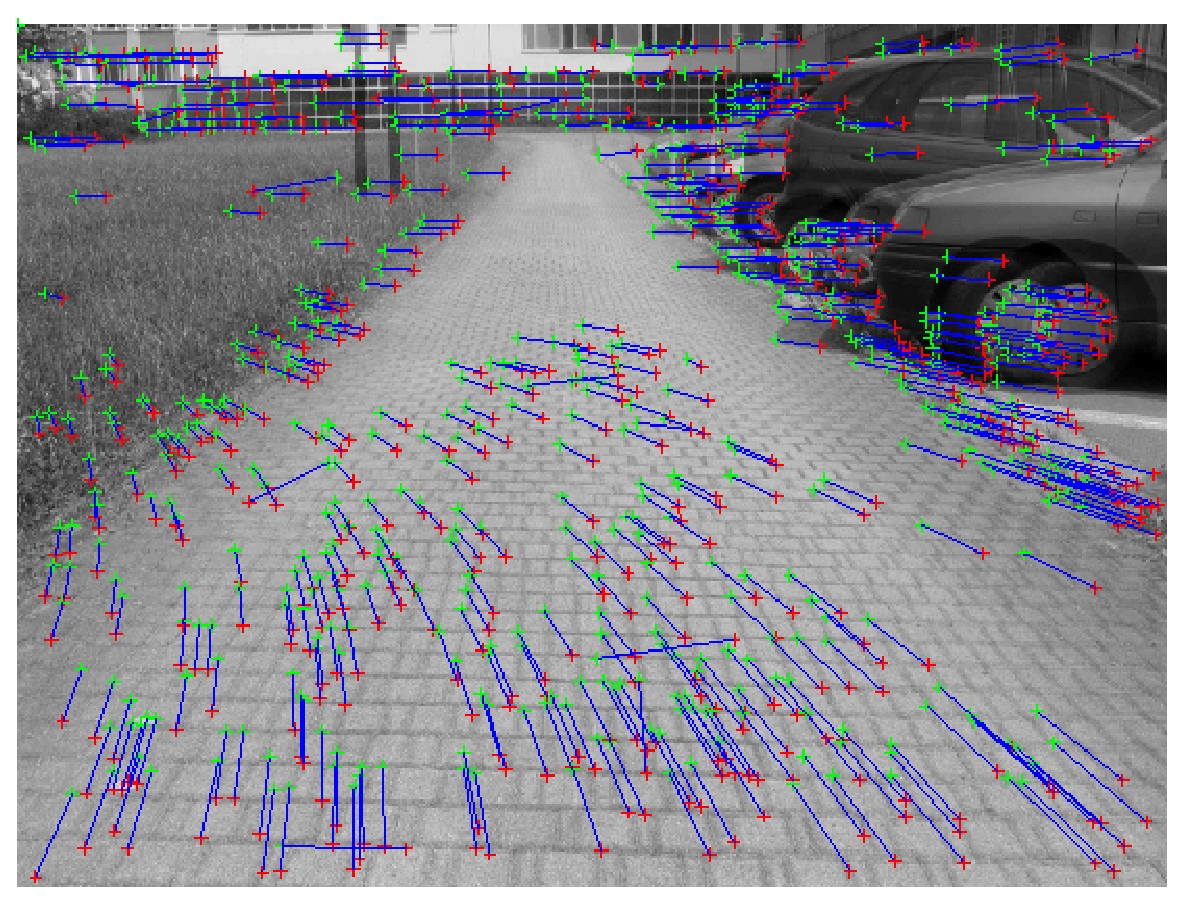
\includegraphics[width=0.48\textwidth]{images/cap2/OdometriaVisual.eps}
  \end{center}
  \vspace{-20pt}
  \caption{Disparidad en odometría visual}
  \vspace{-10pt}
  \label{fig:OdometriaVisual}
\end{wrapfigure}

Pero a partir de las imágenes ¿cómo se puede determinar la distancia de un
objeto respecto al robot? En función del tamaño del objeto en la escena. En un
sistema estereoscópico se comparan la diferencia respecto al eje x (disparidad)
entre la imagen izquierda y derecha. La distancia de un objeto es inversamente
proporcional a la disparidad presente, es decir, si un objeto presenta una gran
disparidad en la escena significa que se encuentra cerca. Cuanto más lejano esté
el objeto la disparidad será menor \cite{OdometriaVisual}.

Por otra parte, en los sistemas con una sóla cámara, también es posible hallar
la distancia. La cámara debe estar orientada hacia el suelo en un ángulo
determinado y a una altura conocida, a partir de la tangente se puede calcular
la distancia.

La odometría visual es la alternativa utilizada en robots móviles que no cuentan
con ruedas: androides, robots voladores, etc. y en los sistemas que no pueden
permitirse el uso de láseres. Aunque es bastante frecuente encontrar la
odometría visual junto a cualquiera de las otras odometrías como apoyo.

La odometría visual cuenta con los siguientes inconvenientes a tener en cuenta:

\begin{itemize}
  \item \textbf{Las cámaras:} para funcionar correctamente, es necesario que las
  cámaras estén calibradas. Por otra parte, si se utiliza un sistema
  estereoscópico se necesita verificar que la distancia entre las cámaras sea la
  correcta.
  \item \textbf{El entorno:} las cámaras son muy sensibles a los cambios bruscos
  de las condiciones del entorno como la luminosidad. También hay que tener en
  cuenta que las escenas son dinámicas, por lo que muchos objetos aparecen y
  desparecen de la escena o se mueven con mucha frecuencia en la escena, y esto
  puede suponer un importante problema.
\end{itemize}
    
Tanto la odometría mecánica, láser y visual presentan varios problemas para
estimar la posición y orientación del robot, sin embargo, combinando ambas se
pueden conseguir resultados más consistentes. Por ejemplo: en aquellos casos
donde la odometría mecánica no coincide con los datos visuales debido a una
superficie inconsistente, se confía en la odometría visual. Por otra parte,
cuando las condiciones lumínicas no son adecuadas en espacios cerrados, se
confía en la odometría láser o mecánica.

%++++++++++++++++++++++++++++++++++++++++++++++++++++++++++++++++++++++++++++++


%++++++++++++++++++++++++++++++++++++++++++++++++++++++++++++++++++++++++++++++
\section{Navegación robótica}
\label{2:sec:4}
%%%%%%%%%%%%%%%%%%%%%%%%%%%%%%%%%%%%%%%%%%%%%%%%%%%%%%%%%%%%%%%%%%%%%%%%%%%%%%%%
% Chapter 2: Conceptos
%%%%%%%%%%%%%%%%%%%%%%%%%%%%%%%%%%%%%%%%%%%%%%%%%%%%%%%%%%%%%%%%%%%%%%%%%%%%%%%%

%+++++++++++++++++++++++++++++++++++++++++++++++++++++++++++++++++++++++++++++++
% \section{Navegación robótica}
% \label{2:sec:4}
% https://en.wikipedia.org/wiki/Mobile_robot_navigation
La navegación robótica es la habilidad que permite a un robot móvil poder
localizarse en el entorno y poder moverse libremente por el mismo, a partir del
conocimiento extraído de las imágenes obtenidas del medio. El objetivo principal
es conocer por donde debe y no debe navegar con la idea de poder alcanzar un
punto de destino marcado previamente. 

En la robótica móvil es indispensable saber como moverse por el mundo, además de
conocer que situaciones de riesgo se han de evitar: colisiones, superficies
irregulares, zonas prohibidas, etc. 

Es posible subdividir la navegación dependiendo de la zona de estudio: de
interiores o de exteriores. En ambos casos las tecnologías pueden ser las
mismas, sin embargo mientras que en la localización en exteriores se suele hacer
uso de GPS, odometría mecánica, etc., en interiores es posible conseguir mejores
resultados con sensores ópticos como cámaras, odometría láser, etc.

La navegación robótica se caracteriza por estos tres tópicos:

\begin{itemize}
  \item \textbf{Localización:} localizarse en el entorno. 
  \item \textbf{Búsqueda de caminos:} búsqueda del camino más optimo para llegar
  a un objetivo. 
  \item \textbf{Mapeo robótico:} construcción de un mapa del entorno. 
\end{itemize}% nube de puntos

%+++++++++++++++++++++++++++++++++++++++++++++++++++++++++++++++++++++++++++++++
\subsection{Localización}
% http://www-math.mit.edu/~hajiagha/cars-fof.pdf
% http://ieeexplore.ieee.org/xpl/login.jsp?tp=&arnumber=1241767&url=http%3A%2F%2Fieeexplore.ieee.org%2Fxpls%2Fabs_all.jsp%3Farnumber%3D1241767

La localización es el primer tema a abordar en la navegación de un robot. El
objetivo es dar respuesta al '¿dónde estoy?', a través de conocer la posición
inicial, conocer la posición del punto de destino y autolocalizarse por el
entorno. La localización se puede dividir en dos grupos principales: basada en
puntos de referencias y basada en el análisis de las imágenes.

La localización basada en puntos de referencias se aprovecha en los puntos de
referencias que existen en el entorno y sobresalen de las imágenes de la escena
sin verse influenciados por otros factores de las escenas como los cambios en el
entorno o de los elementos que lo componen. Este tipo de puntos o marcas pueden
ser artificiales (líneas o flechas en un mapa o GPS) o naturales (puertas,
esquinas, senderos, etc.).

\begin{figure}[!th]
  \begin{center}
    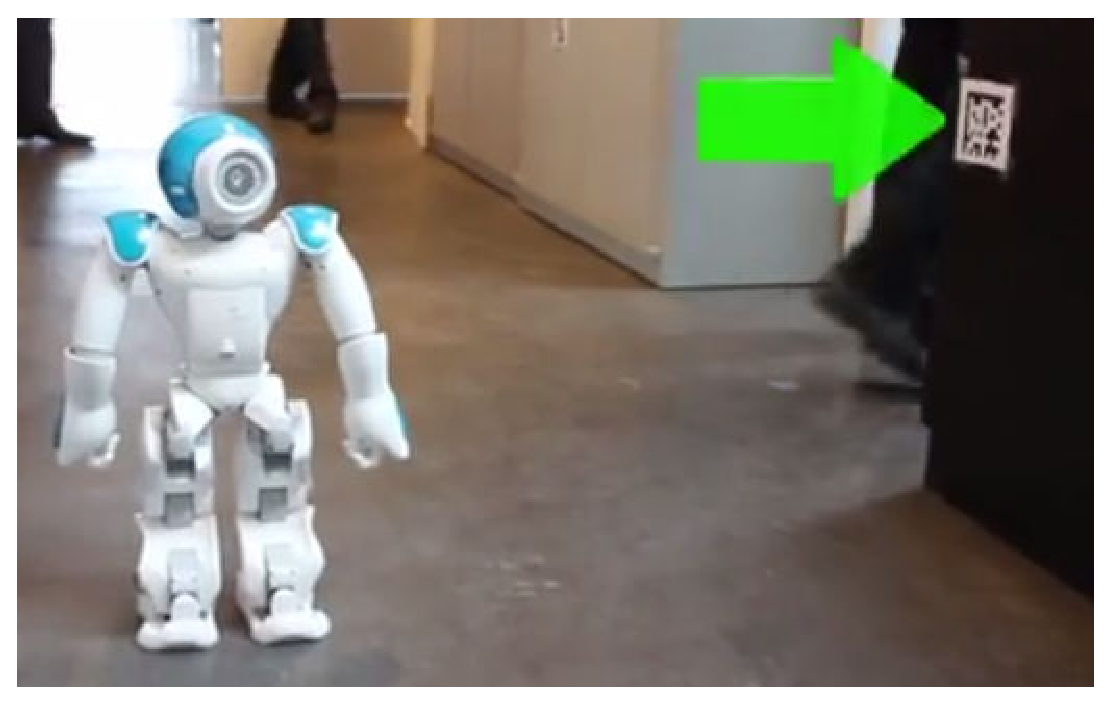
\includegraphics[width=0.5\textwidth]{images/cap2/LocalizacionMarcas.eps}
    \caption{Localización a través de código QR}
    \label{fig:LocalizacionMarcas}
  \end{center}
\end{figure}

Cuando este tipo de marcas no se pueden separar de las imágenes, porque bien no
se tienen puntos de referencia artificiales, o no se puede reconocer del propio
entorno marcas artificiales, se recurre a la localización basada en el análisis
de las imágenes capturadas. El primer paso es el 'auto-aprendizaje',
habitualmente navegar de forma autónoma y recoger las imágenes del entorno.
Estas imágenes se procesan, comparando los elementos en la escena de cada nueva
imagen recogida con la anterior y las imágenes que se tiene en el histórico,
obteniendo así la localización actual.

\begin{figure}[!th]
  \begin{center}
    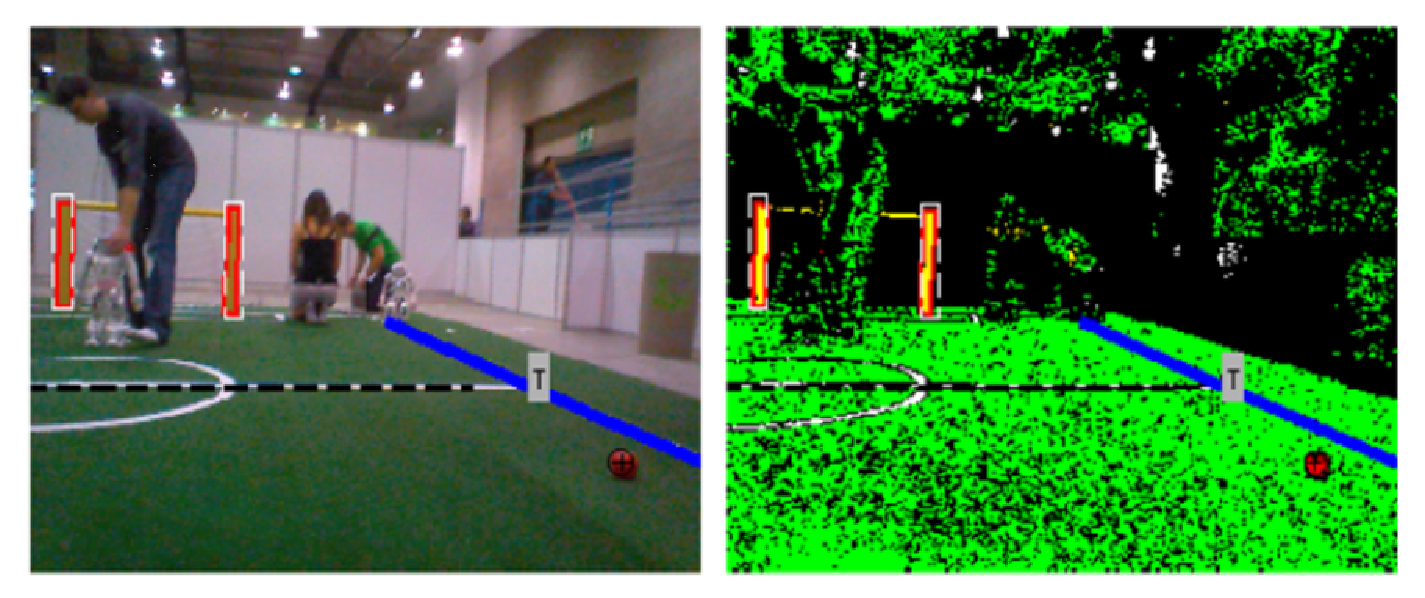
\includegraphics[width=0.7\textwidth]{images/cap2/LocalizacionImagenes.eps}
    \caption{Localización mediante los elementos de la escena}
    \label{fig:LocalizacionImagenes}
  \end{center}
\end{figure}

%--------------------------------------
\paragraph{Filtro de Kalman Extendido} \hspace{0pt} \\
% http://www.robolabo.etsit.upm.es/~inaki/coursework/kalman.pdf
% http://bibing.us.es/proyectos/abreproy/11879/fichero/PFC+Sergio+Pereira+Ruiz%252F7+-+Filtro+de+Kalman.pdf
% http://www.ual.es/personal/rgonzalez/documents/slam_ramon.pdf
El filtro de Kalman extendido (EKF) es un algoritmo que permite estimar la
posición de un robot a partir de la combinación de las ecuaciones de la
odometría y las medidas recogidas por los sensores. Se trata de un algoritmo muy
utilizado en sistemas de navegación.

El filtro de Kalman se basa en dos etapas: predicción y corrección.

En la etapa de predicción se tiene solamente en cuenta la odometría, cuyos datos
son almacenados en un vector de estado, los cuales se toman como una estimación
Este vector contiene las variables de interés, manteniendo el tiempo dos
posibles valores: el valor previsto (a priori) y el valor corregido (a
posteriori).

En la etapa de corrección, se introducen las medidas de los sensores. Con  la
odometría y los sensores, se calcula la diferencia entre el valor esperado y el
real, se obtiene la matriz de covarianza del sensor y se obtiene la Ganancia de
Kalman (determina cuanto se debe corregir la estimación). Finalmente se corrigen
los valores del vector de estado después de las nuevas observaciones.

Conforme pasa el tiempo crece la imprecisión, por lo que las etapas se repiten
sucesivamente con el fin de reducir la imprecisión.

\begin{figure}[!th]
  \begin{center}
    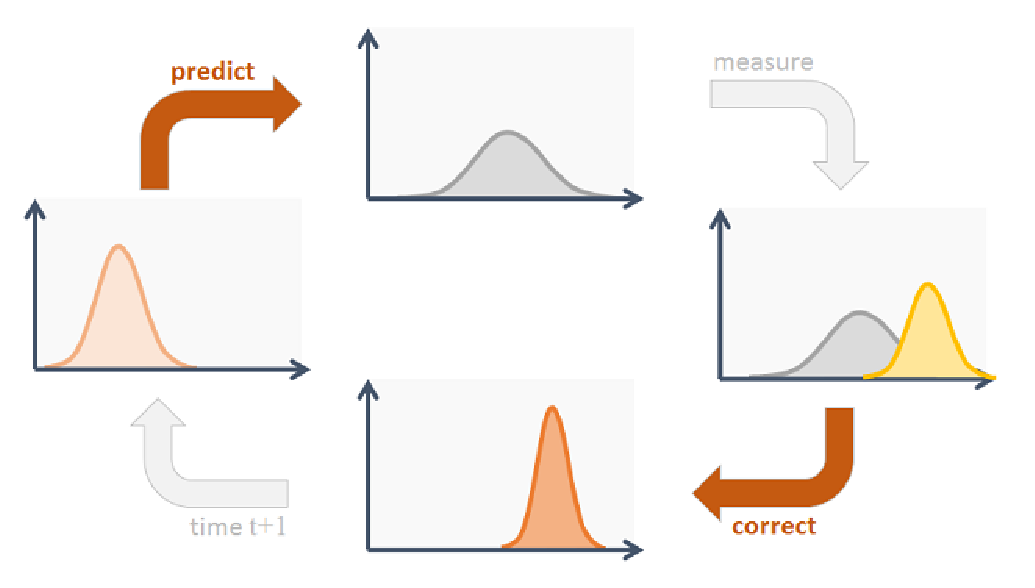
\includegraphics[width=0.7\textwidth]{images/cap2/Kalman.eps}
    \caption{Esquema del filtro de Kalman extendido}
    \label{fig:Kalman}
  \end{center}
\end{figure}

%+++++++++++++++++++++++++++++++++++++++++++++++++++++++++++++++++++++++++++++++
\subsection{Búsqueda de caminos}
% https://en.wikipedia.org/wiki/Motion_planning
% http://correll.cs.colorado.edu/?p=965111
% http://ais.informatik.uni-freiburg.de/teaching/ss11/robotics/slides/18-robot-motion-planning.pdf
% http://rabida.uhu.es/dspace/bitstream/handle/10272/5501/Nuevas_aportaciones_en_algoritmos_de_planificacion.pdf?sequence=2
La búsqueda de caminos permite hallar el conjunto de movimientos que permite a
un robot encontrar el camino más óptico hasta llegar a su objetivo, para no
solamente llegar en el menor tiempo posible, sino también evitar por el camino
los obstáculos que hagan peligrar el estado del robot o simplemente le retrasen.

El problema de la búsqueda de caminos ha sido ampliamente estudiado, existiendo
múltiples algoritmos para solventar este problema. 

Entre los métodos más conocidos están los 'roadmap', los cuales se basan en
construir una descripción de todo el espacio libre en el plano mediante un
grafo. Posteriormente los nodos del grafo se van conectando a partir de las
distancias más cortas entre sí, formando todos los caminos posibles, entre los
que se encuentra el más óptimo.

\begin{figure}[!th]
  \begin{center}
    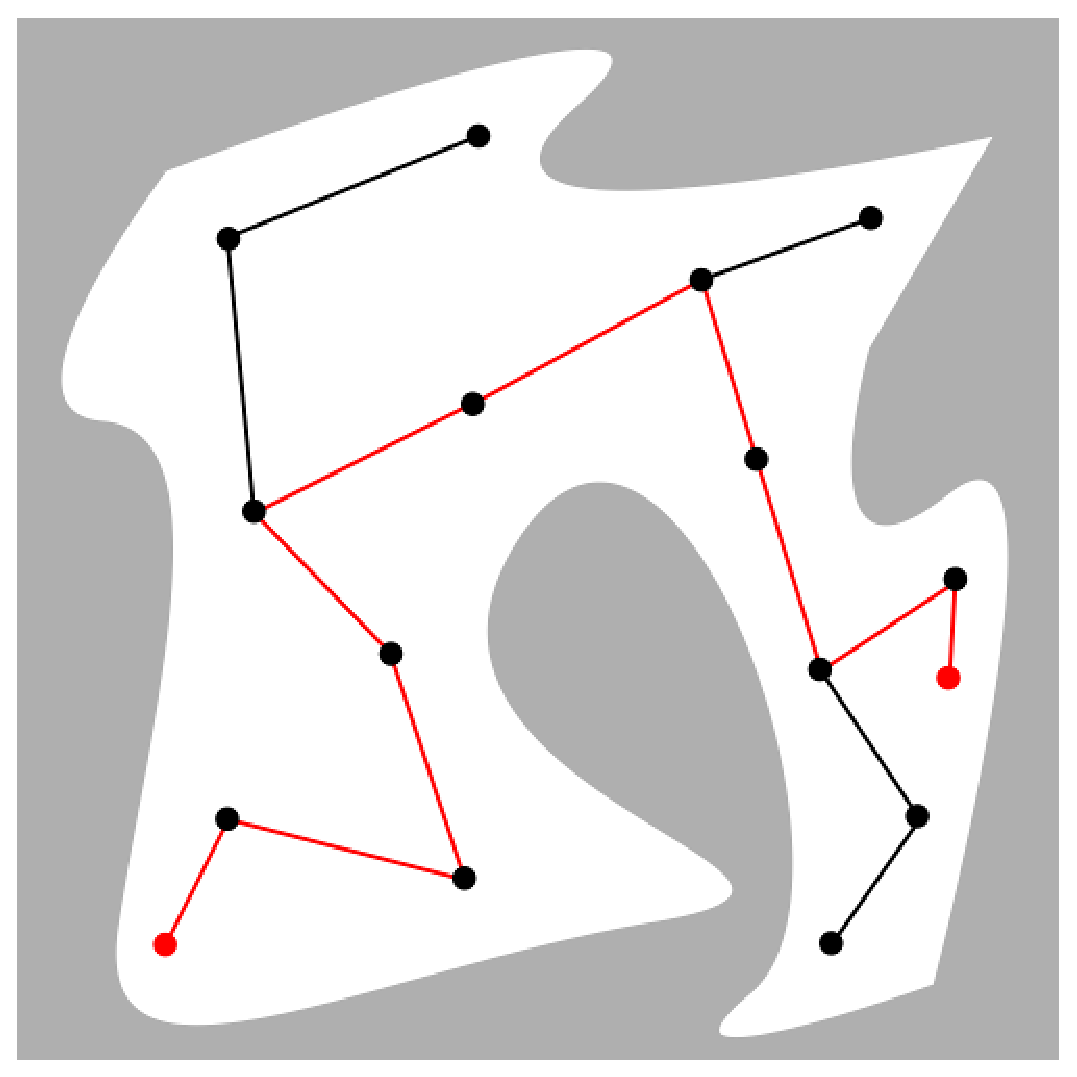
\includegraphics[width=0.5\textwidth]{images/cap2/BusquedaCaminosRoadmap.eps}
    \caption{Ejemplo de un 'roadmap'}
    \label{fig:BusquedaCaminosRoadmap}
  \end{center}
\end{figure}

Por otra parte, existen los métodos de descomposición en celdas, que en vez de
representar el entorno en un grafo, dividen el espacio libre de colisiones en un
conjunto de celdas. 

En los últimos años han surgido métodos alternativos que permiten dar solución a
la complejidad del entornos y las restricciones cinemáticas que puede presentar
un robot en la búsqueda de caminos, son los algoritmos de generación aleatoria,
el más famoso es el RRT o 'Rapidly Exploring Random Trees', muy utilizados en la
navegación autónoma. Este algoritmo se basa en la construcción al azar de un 
árbol que va creciendode manera incremental mediante la captura de nuevas
muestras del entorno.

%+++++++++++++++++++++++++++++++++++++++++++++++++++++++++++++++++++++++++++++++
\subsection{Mapeo robótico}
% https://en.wikipedia.org/wiki/Robotic_mapping
% https://en.wikipedia.org/wiki/3D_reconstruction_from_multiple_images
% Introduccion sobre el mapeo en robotica, que es porque...

La construcción de un mapa constituye el objetivo final de la navegación
robótica. Al igual que en la cartografía, un mapa representa toda la información
conocida acerca de un entorno: dimensiones del entorno, orografía, localización
de los obstáculos, etc. En robótica la utilización de un mapa es de gran
utilidad ya que permite tener un registro histórico de aquellas lugares que ya
ha visitado en el pasado, evitando así visitar zonas peligrosas o irrelevantes.

Los mapas se pueden representar de diferentes formas:

\begin{itemize}
  \item \textbf{Mapa métrico:} representación bidimensional del espacio y todos
  los objetos que lo rodean. Aunque la posición de los obstáculos es bastante
  aproximada a la realidad, deja de lado información importante del entorno. Una
  ampliacion de este tipo de mapas es mediante una representación tridimensional
  a través de la disposición de una nube de puntos, siendo posible apreciar
  datos  importantes del entorno: orografía del terreno, altura de los
  obstáculos, imágenes más detalladas del entorno, etc.
  \item \textbf{Mapa topológico:} grafo en el que los nodos corresponden a los
  lugares y sus arcos a la distancia entre ellos. Permite tener un abstracto
  claro y sencillo de la relación de los obstáculos entre ellos.
\end{itemize}

%--------------------------------------
\paragraph{SLAM} \hspace{0pt}

% http://www.ual.es/personal/rgonzalez/documents/slam_ramon.pdf
% https://es.wikipedia.org/wiki/SLAM_%28rob%C3%B3tica%29
% http://ais.informatik.uni-freiburg.de/teaching/ss12/robotics/slides/12-slam.pdf
A pesar de que la navegación de un robot se ha divido en tres etapas, donde la
primera es la localización y la última lo construcción de un mapa, realmente un
robot autónomo es capaz de construir un mapa del entorno comenzando desde una
posición desconocida en el mismo.

SLAM (Simultaneous Localization And Mapping) es una técnica que permite a un
robot construir un mapa de un entorno desconocido a la vez que es capaz de
localizarse en el mismo mediane sus sensores. 

Uno de los factores más importantes a tener en cuenta es la incertidumbre: no se
conoce ni la posición ni el entorno, y no solo eso, los sensores no son
perfectos y pueden arrojar resultados que no son acordes a la realidad,  por lo
que la clave está en seguir un modelo probabilístico. Esta imprecisión puede
corregirse con el paso del tiempo recorriendo continuadamente.

% algo mas tecnico
% loop closure

SLAM toma como base el teorema de Bayes para dar solución del problema, mediante
el uso de algritmos como el Filtro de Kalman Extendido o los Mapas de ocupación
de eldillas. Por otra parte, uno de los retos a los que se enfrenta SLAM es al
'loop closure' (cierre de bucle). Se trata del problema de reconocer aquel lugar
del mapa que ya ha sido visitado previamente. El éxito del SLAM depende poder
detectar esta situación

Los principales problemas con los que cuenta SLAM radican en la complejidad que
se tiene en los entornos dinámicos donde muchos objetos en el mapa se mueven
libremente. Por otra parte, es una técnica muy exigente que no se puede utilizar
en grandes entornos con muchos objetos, ya que el coste computacional crece al
cuadrado conforme a los objetos contenidos en el mapa.

A pesar de ello, los resultados obtenidos por SLAM son muy atractivos, ya que
sin conocer ni la posición ni el mapa, un robot autónomo puede moverse
libremente por el, obteniendo al mismo tiempo un mapa del entorno. Por otra
parte esta técnica es bastante robusta ante el ruido provocado por lo sensores.

%++++++++++++++++++++++++++++++++++++++++++++++++++++++++++++++++++++++++++++++


%++++++++++++++++++++++++++++++++++++++++++++++++++++++++++++++++++++++++++++++
